\documentclass{standalone}
\usepackage{tikz}
\begin{document}
% TI-84 style calculator screen, 4:3 aspect ratio (8cm x 6cm).
% Window: x in [-4.5,6.5], y in [-6,10].
% Function: y = |5/6 (x+3)(x-5) + 5| - 5
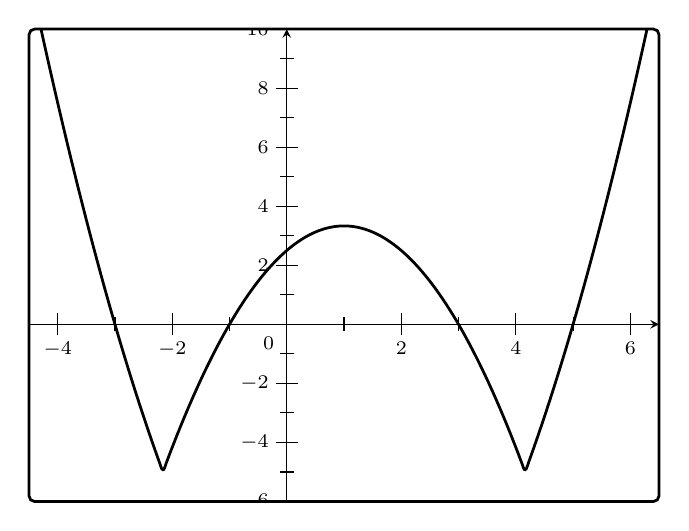
\begin{tikzpicture}[x=0.72727cm, y=0.375cm, >=stealth]
  % screen border (exactly the viewing window -> 4:3)
  \draw[rounded corners=2pt, line width=1pt] (-4.5,-6) rectangle (6.5,10);

  \begin{scope}
    \clip (-4.5,-6) rectangle (6.5,10);

    % axes
    \draw[->] (-4.5,0) -- (6.5,0);
    \draw[->] (0,-6) -- (0,10);

    % minor tick marks (every 1 unit)
    \foreach \x in {-3,-1,1,3,5}
      \draw ([yshift=-2.5pt]\x,0) -- ([yshift=2.5pt]\x,0);
    \foreach \y in {-5,-3,-1,1,3,5,7,9}
      \draw ([xshift=-2.5pt]0,\y) -- ([xshift=2.5pt]0,\y);

    % major tick marks (every 2 units) with labels
    \foreach \x in {-4,-2,2,4,6} {
      \draw ([yshift=-4pt]\x,0) -- ([yshift=4pt]\x,0);
      \node[below=3pt] at (\x,0) {\scriptsize $\x$};
    }
    \foreach \y in {-6,-4,-2,2,4,6,8,10} {
      \draw ([xshift=-4pt]0,\y) -- ([xshift=4pt]0,\y);
      \node[left=3pt] at (0,\y) {\scriptsize $\y$};
    }
    \node[below left=1pt] at (0,0) {\scriptsize $0$};

    % curve: y = |5/6 (x+3)(x-5) + 5| - 5
    \draw[line width=1pt, smooth, samples=300, domain=-4.5:6.5]
      plot (\x, {abs(5/6*(\x+3)*(\x-5) + 5) - 5});
  \end{scope}
\end{tikzpicture}
\end{document}
